\chapter{Sequence diagrams}

\section{Data Acquisition}
\begin{figure}[!ht]
	\begin{center}
		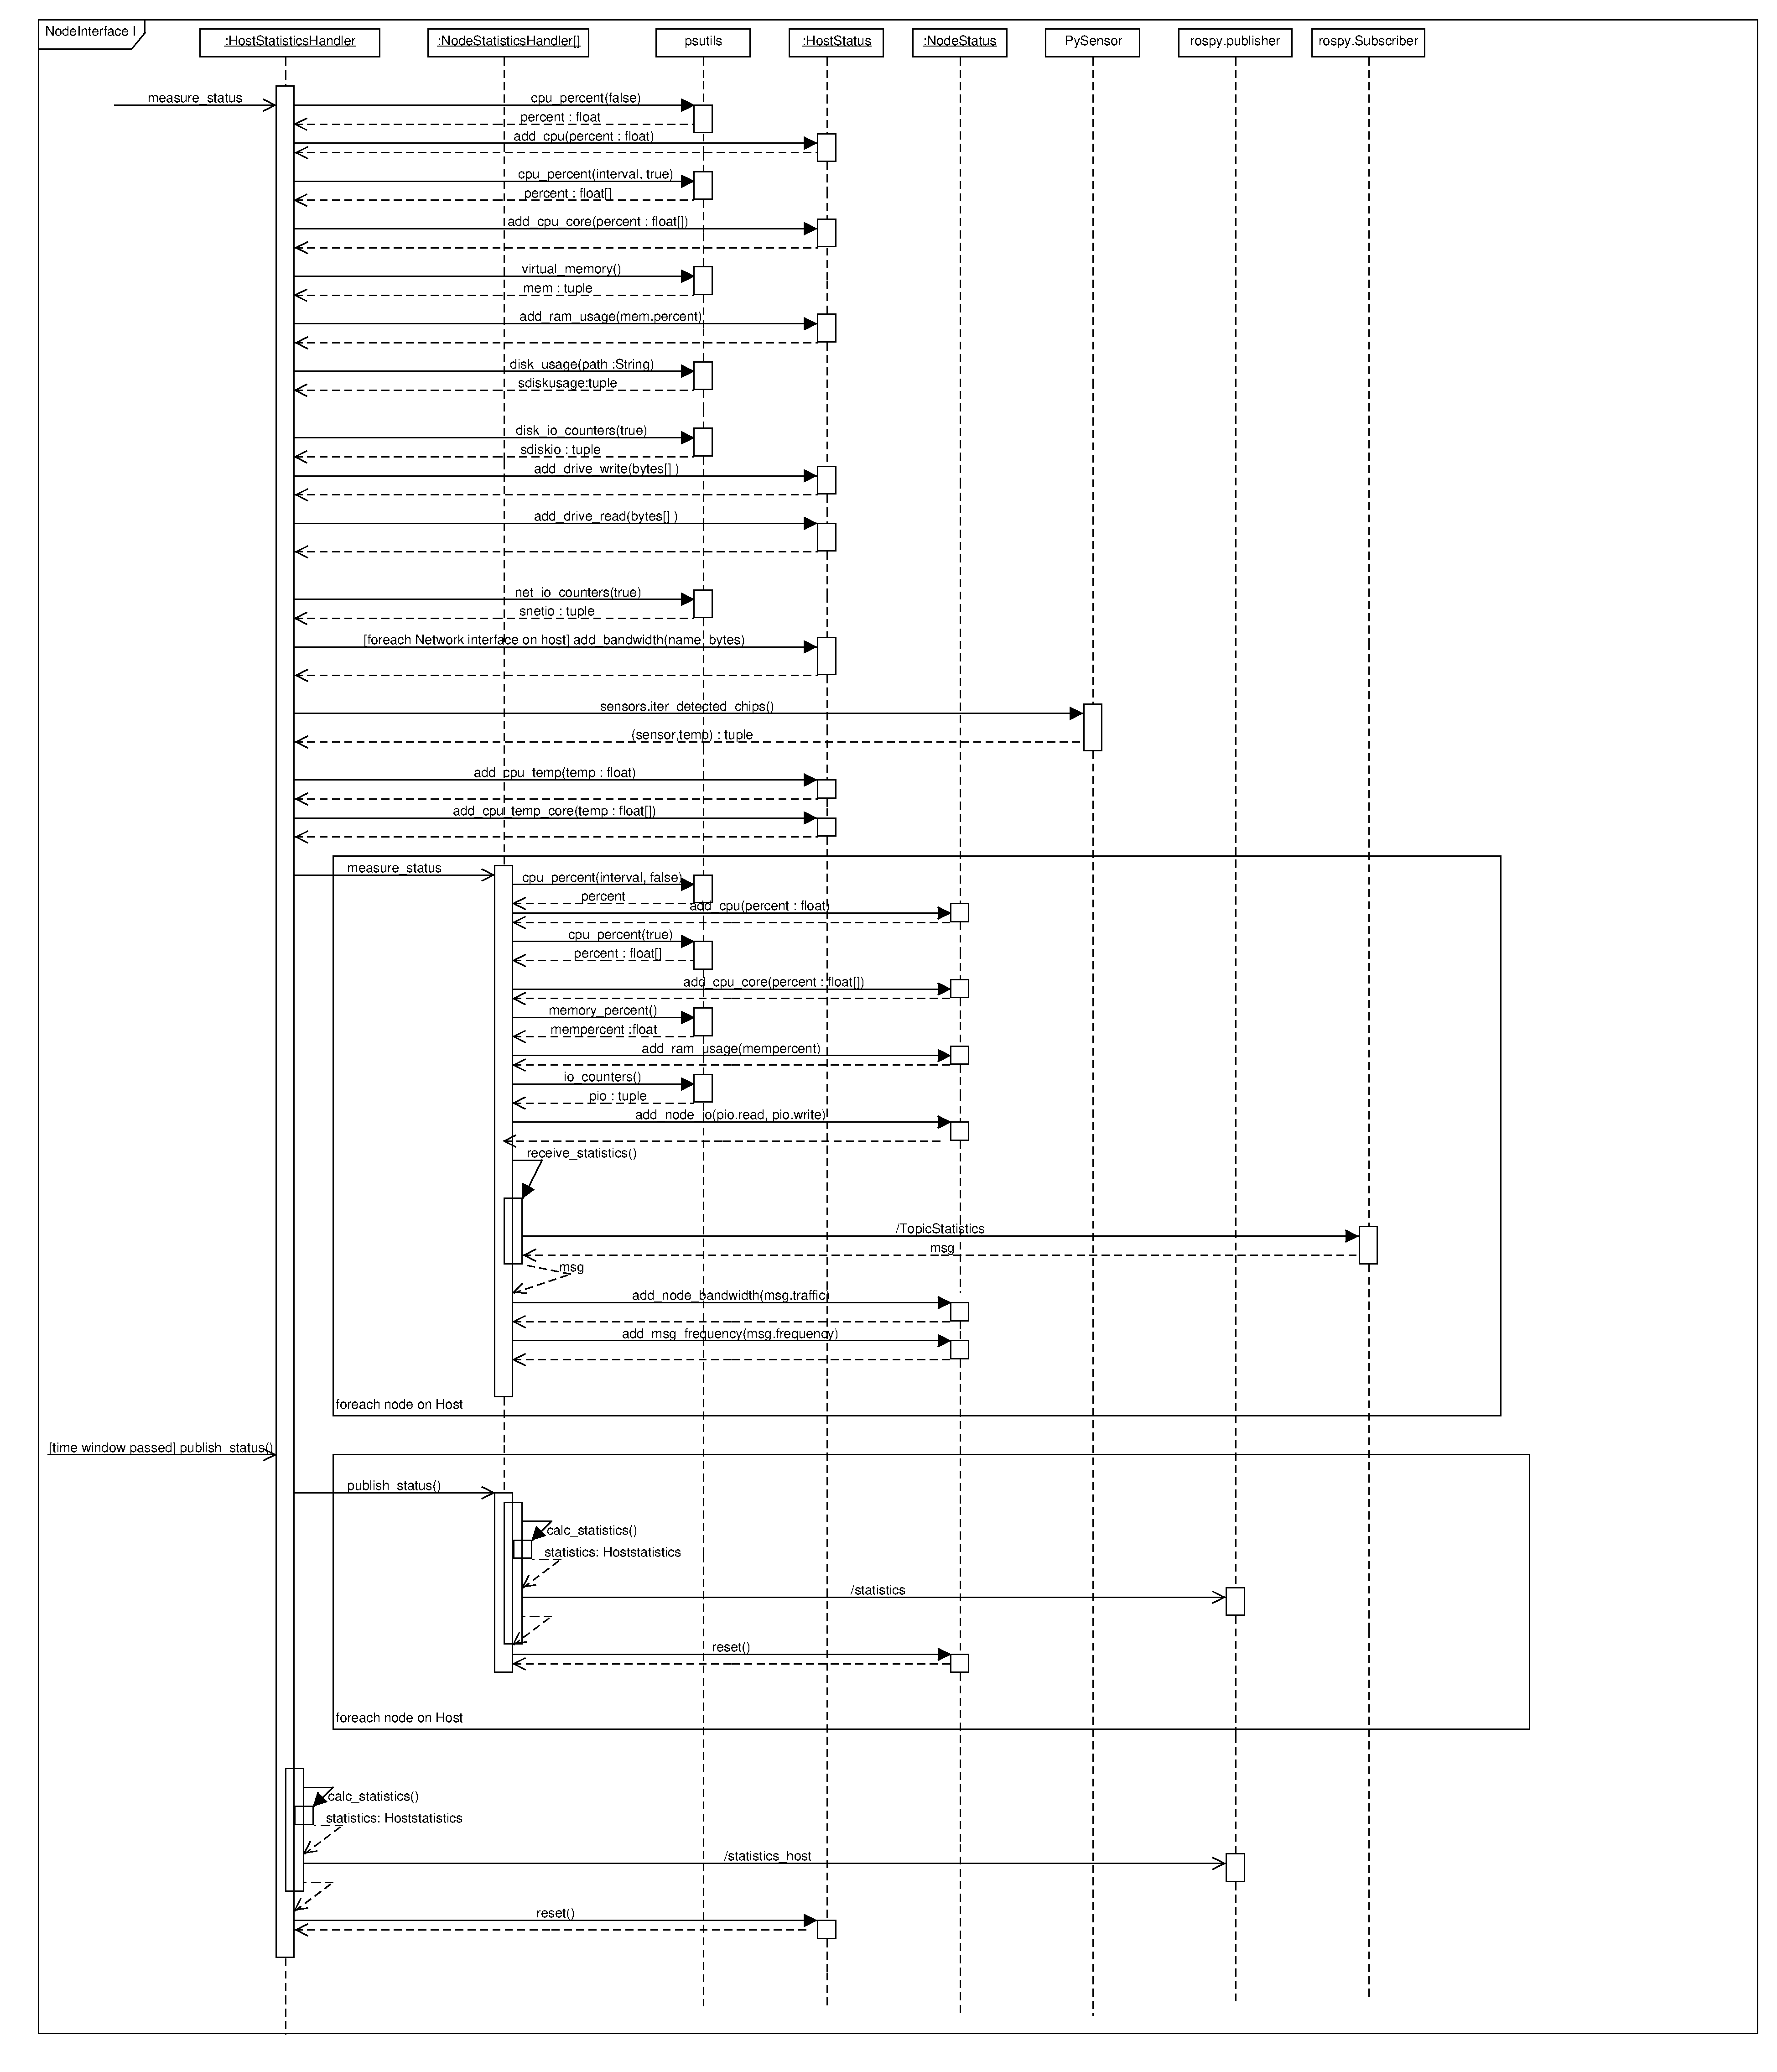
\includegraphics[width=0.8\linewidth]{./diagram_pictures/NodeInterface/erfassung_seq.pdf}
		\caption{Used psutils calls to collect data and publishing to topics.}
	\end{center}
\end{figure}

\subsection{Acquisition}
The Acquisition is triggered by a timer. The HostStatisticsHandler uses psutils and PySensors to collect data about it's current state and write it into the HostStatus instance. It also triggers an asynchronous call of measure\_status to all of it's node's executed in individual threads.
The nodes use psutils and ROS Topic Statistics to collect data and write it into the NodeStatus instance.

\subsection{Publishing}
After the time window has passed the publishing process is triggered. The HostStatisticsHandler again triggers asynchronous calls to all of it's nodes to publish their status. During the publishing process, the statistical values are calculated and transformed into a ROS message.
After publishing the data, the status of the host or node is resetted.

\newpage
\section{Dataprocessing and -storage}
\begin{figure}[!ht]
	\begin{center}
		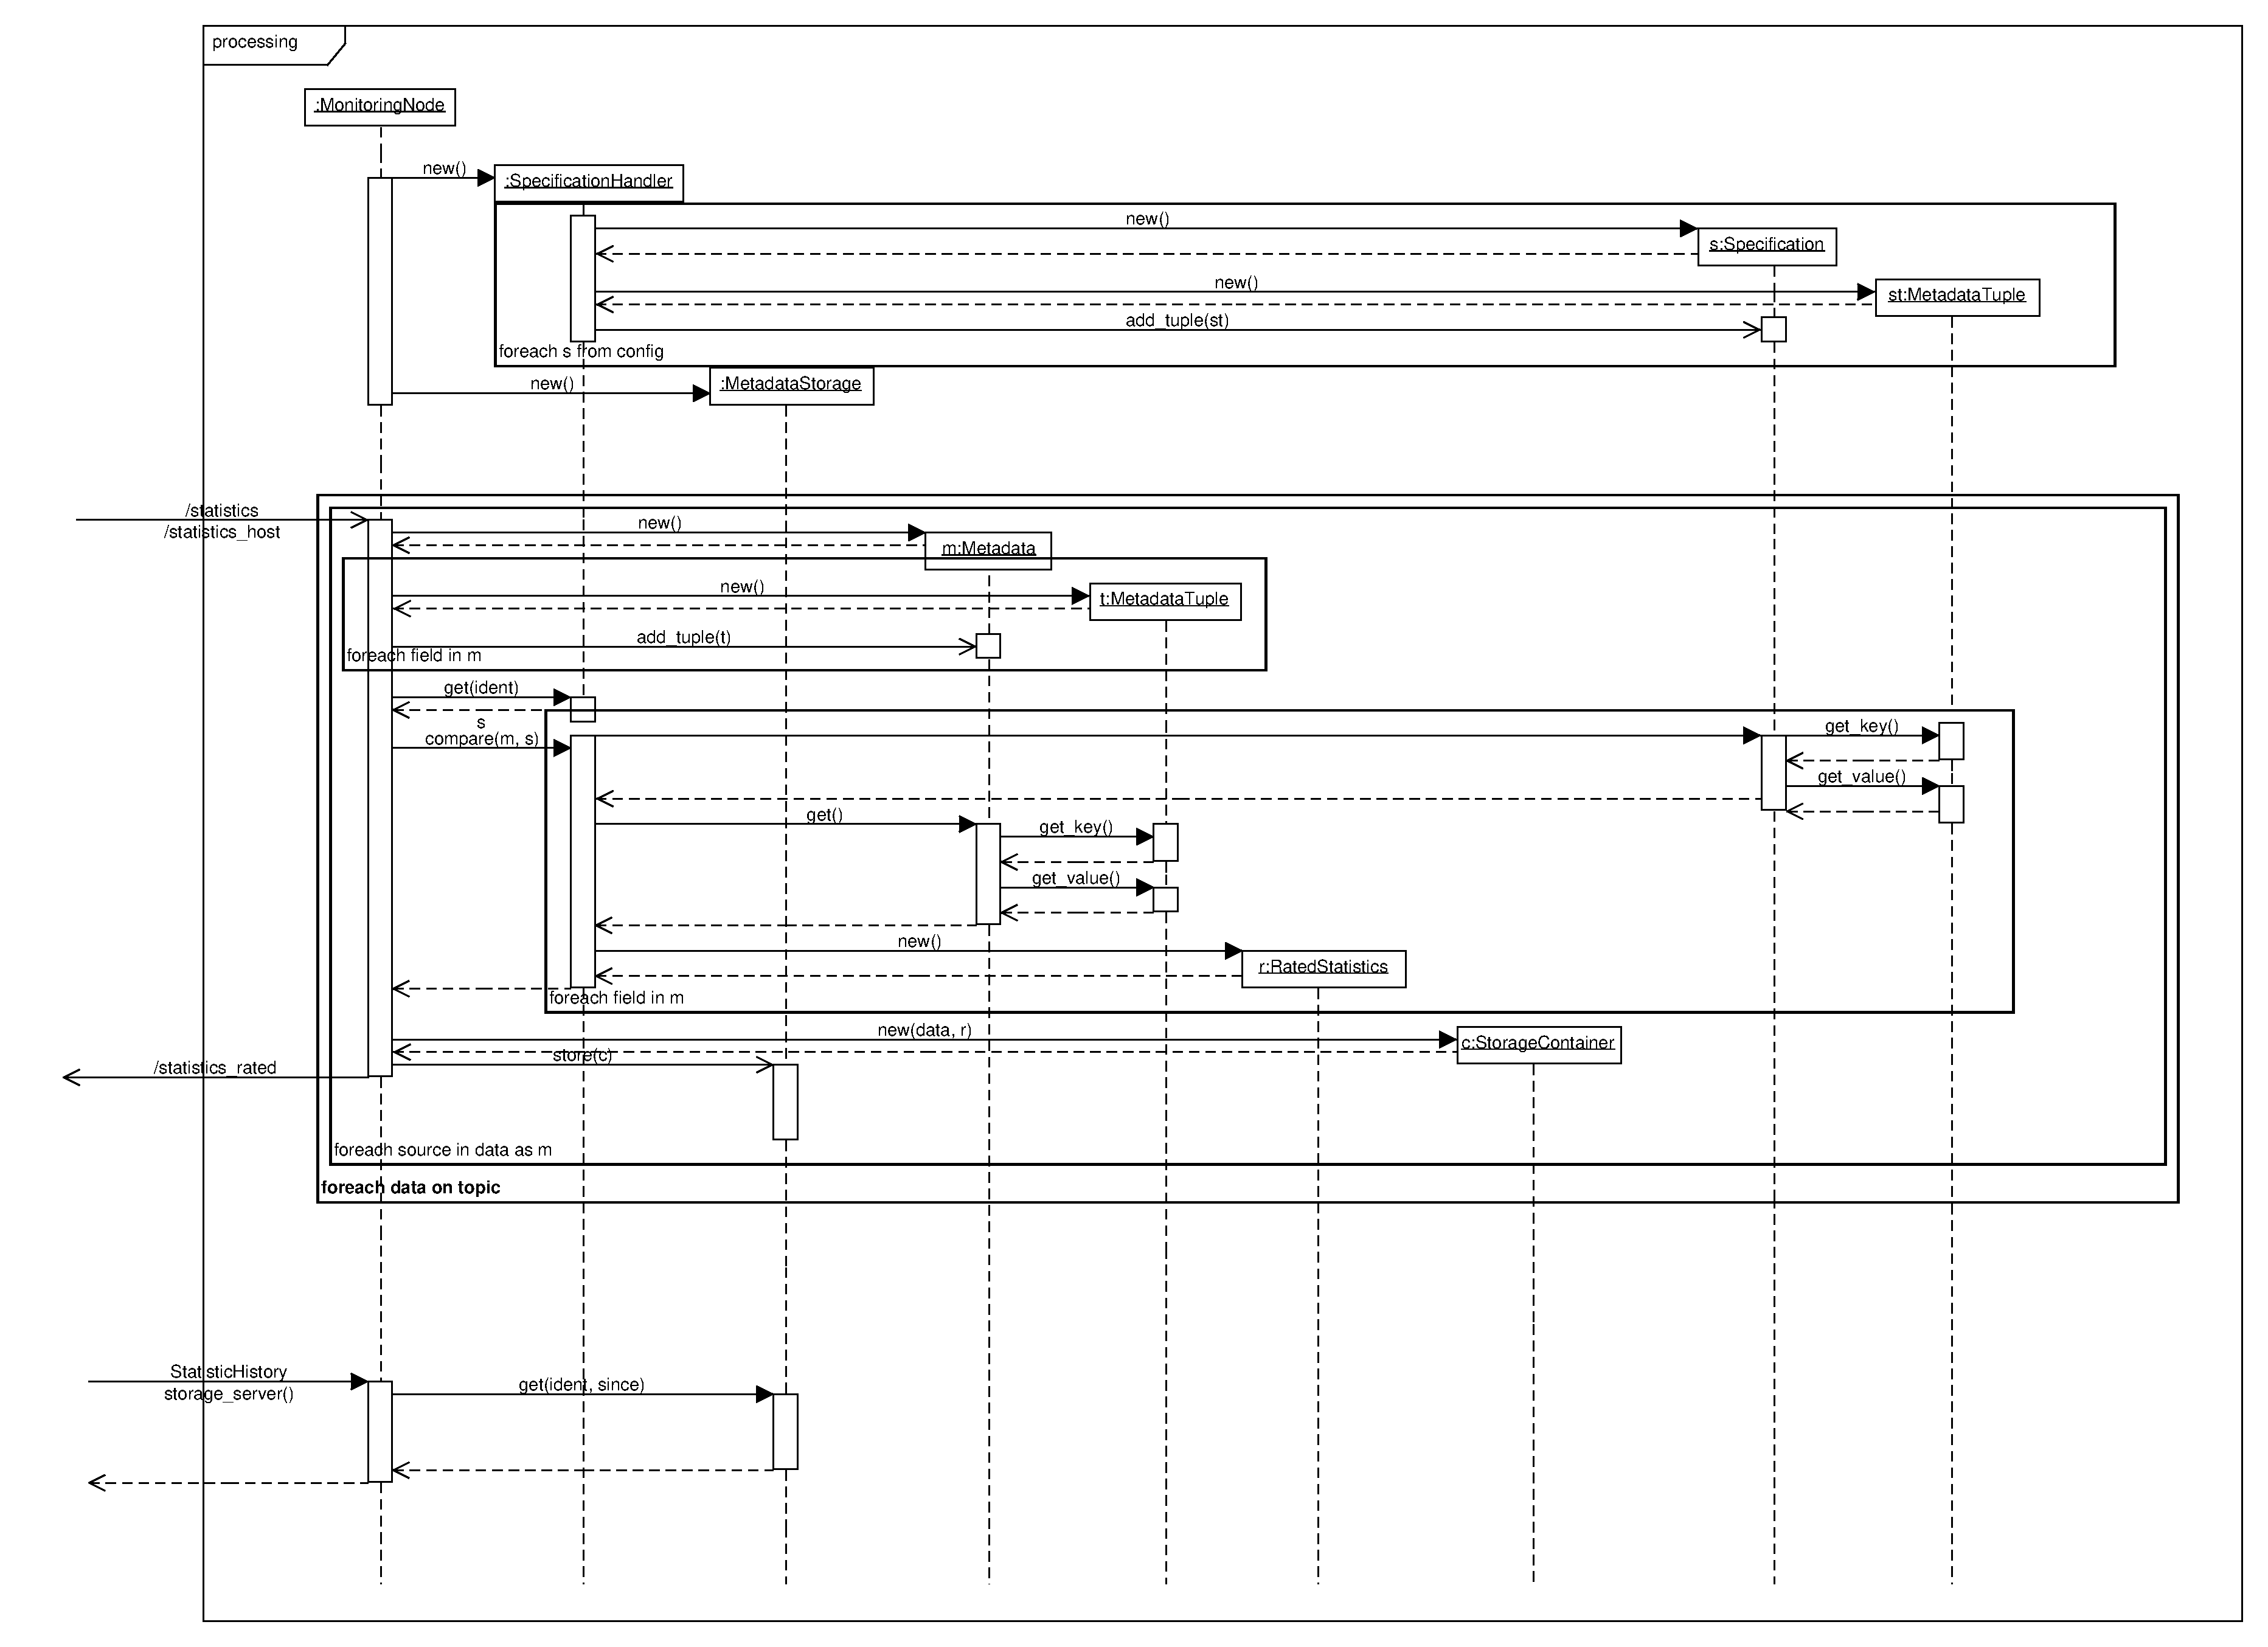
\includegraphics[width=1.0\linewidth]{./diagram_pictures/processing_seq.pdf}
		\caption{Three sequences appearing in the data-processing part of the project.}
	\end{center}
\end{figure}

\subsection*{Setup}
During the first activity of the MonitoringNode, it sets up a SpecificationHandler, which then loads all specifications from config files and stores them in MetadataTuple objects bundled in Specification objects.\\
It then sets up the MetadataStorage.

\subsection*{Receiving data}
The second activity of the MonitoringNode is triggered on receiving data on either the /statistics or /statistics\_host topic. The incoming data is translated into Metadata objects containing of several MetadataTuples describing every measurement featured in the received data.\\
Now the MonitoringNode looks up a Specification from SpecificationHandler concerning the connection/node/host it just received data about.\\
On success it compares the created Metadata object with the found Specification object MetadataTuple-wise for each field featured in the Metadata/Specification object.\\
Erroneous results will be marked in a new RatedStatistics object. Bundled with the raw input data, a timestamp and an identifier describing the concerned connection/node/host it will be stored in the MetadataStorage object created on setup.

\subsection*{Providing data for the GUI}
Answering a request for all data or a special identifier describing a connection/node/host since a given point of time, the MonitoringNode will return the matching data from the MetadataStorage.
A result of that will contain raw data, rated data, a timestamp and the identifier mentioned above.
 
\newpage 
\section{Countermeasures} 
\begin{figure}[!ht] 
	\begin{center} 
		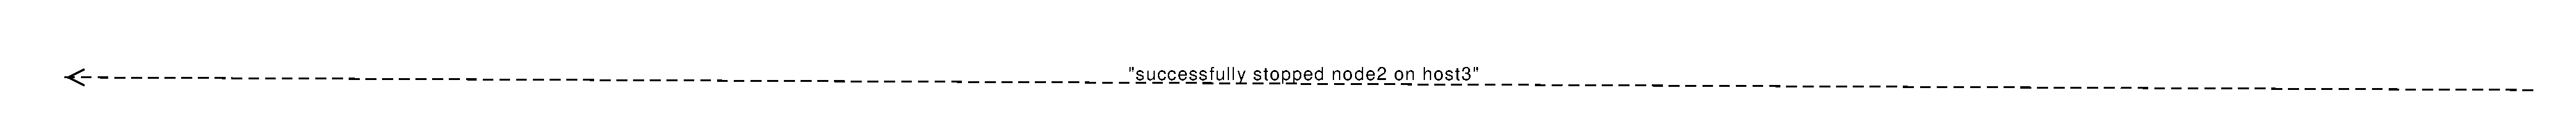
\includegraphics[width=1.0\linewidth]{./diagram_pictures/reactor/reactor_seq.pdf} 
		\caption{Initialisation of Constraints and evaluating and executing countermeasures.} 
	\end{center} 
\end{figure}
This sequence diagram shows how constraints get initialised from the parameter server. Additionally it states how an constraint first gets evaluated periodically and then executes it's reaction when necessary.
\subsection*{Initialisation of Constraints}
First the ConstraintHandler asks for all constraints from the parameter server. Then the class parses them into Constraints, building an tree for efficient evaluation. Each constraint has its own array of reactions to take when necessary.

\subsection*{Evaluation and reacting}
The CountermeasureNode regularily asks the ConstraintHandler to evaluate the constraints again. Each evaluate call in an ConstraintItem gets passed on to the objects branches until the leafes are reached. Each leaf then evaluates if the specific contraint for one specific statistic datapoint is true and passes its result on back on its way to the root of the tree.\\
After the evaluation the ConstraintHandler checks if there is the need to react. The reaction creates a new NodeReaction object and sends it to the remote ReactionHandler.


\newpage
\section{GUI}
\begin{figure}[!ht]
	\begin{center}
		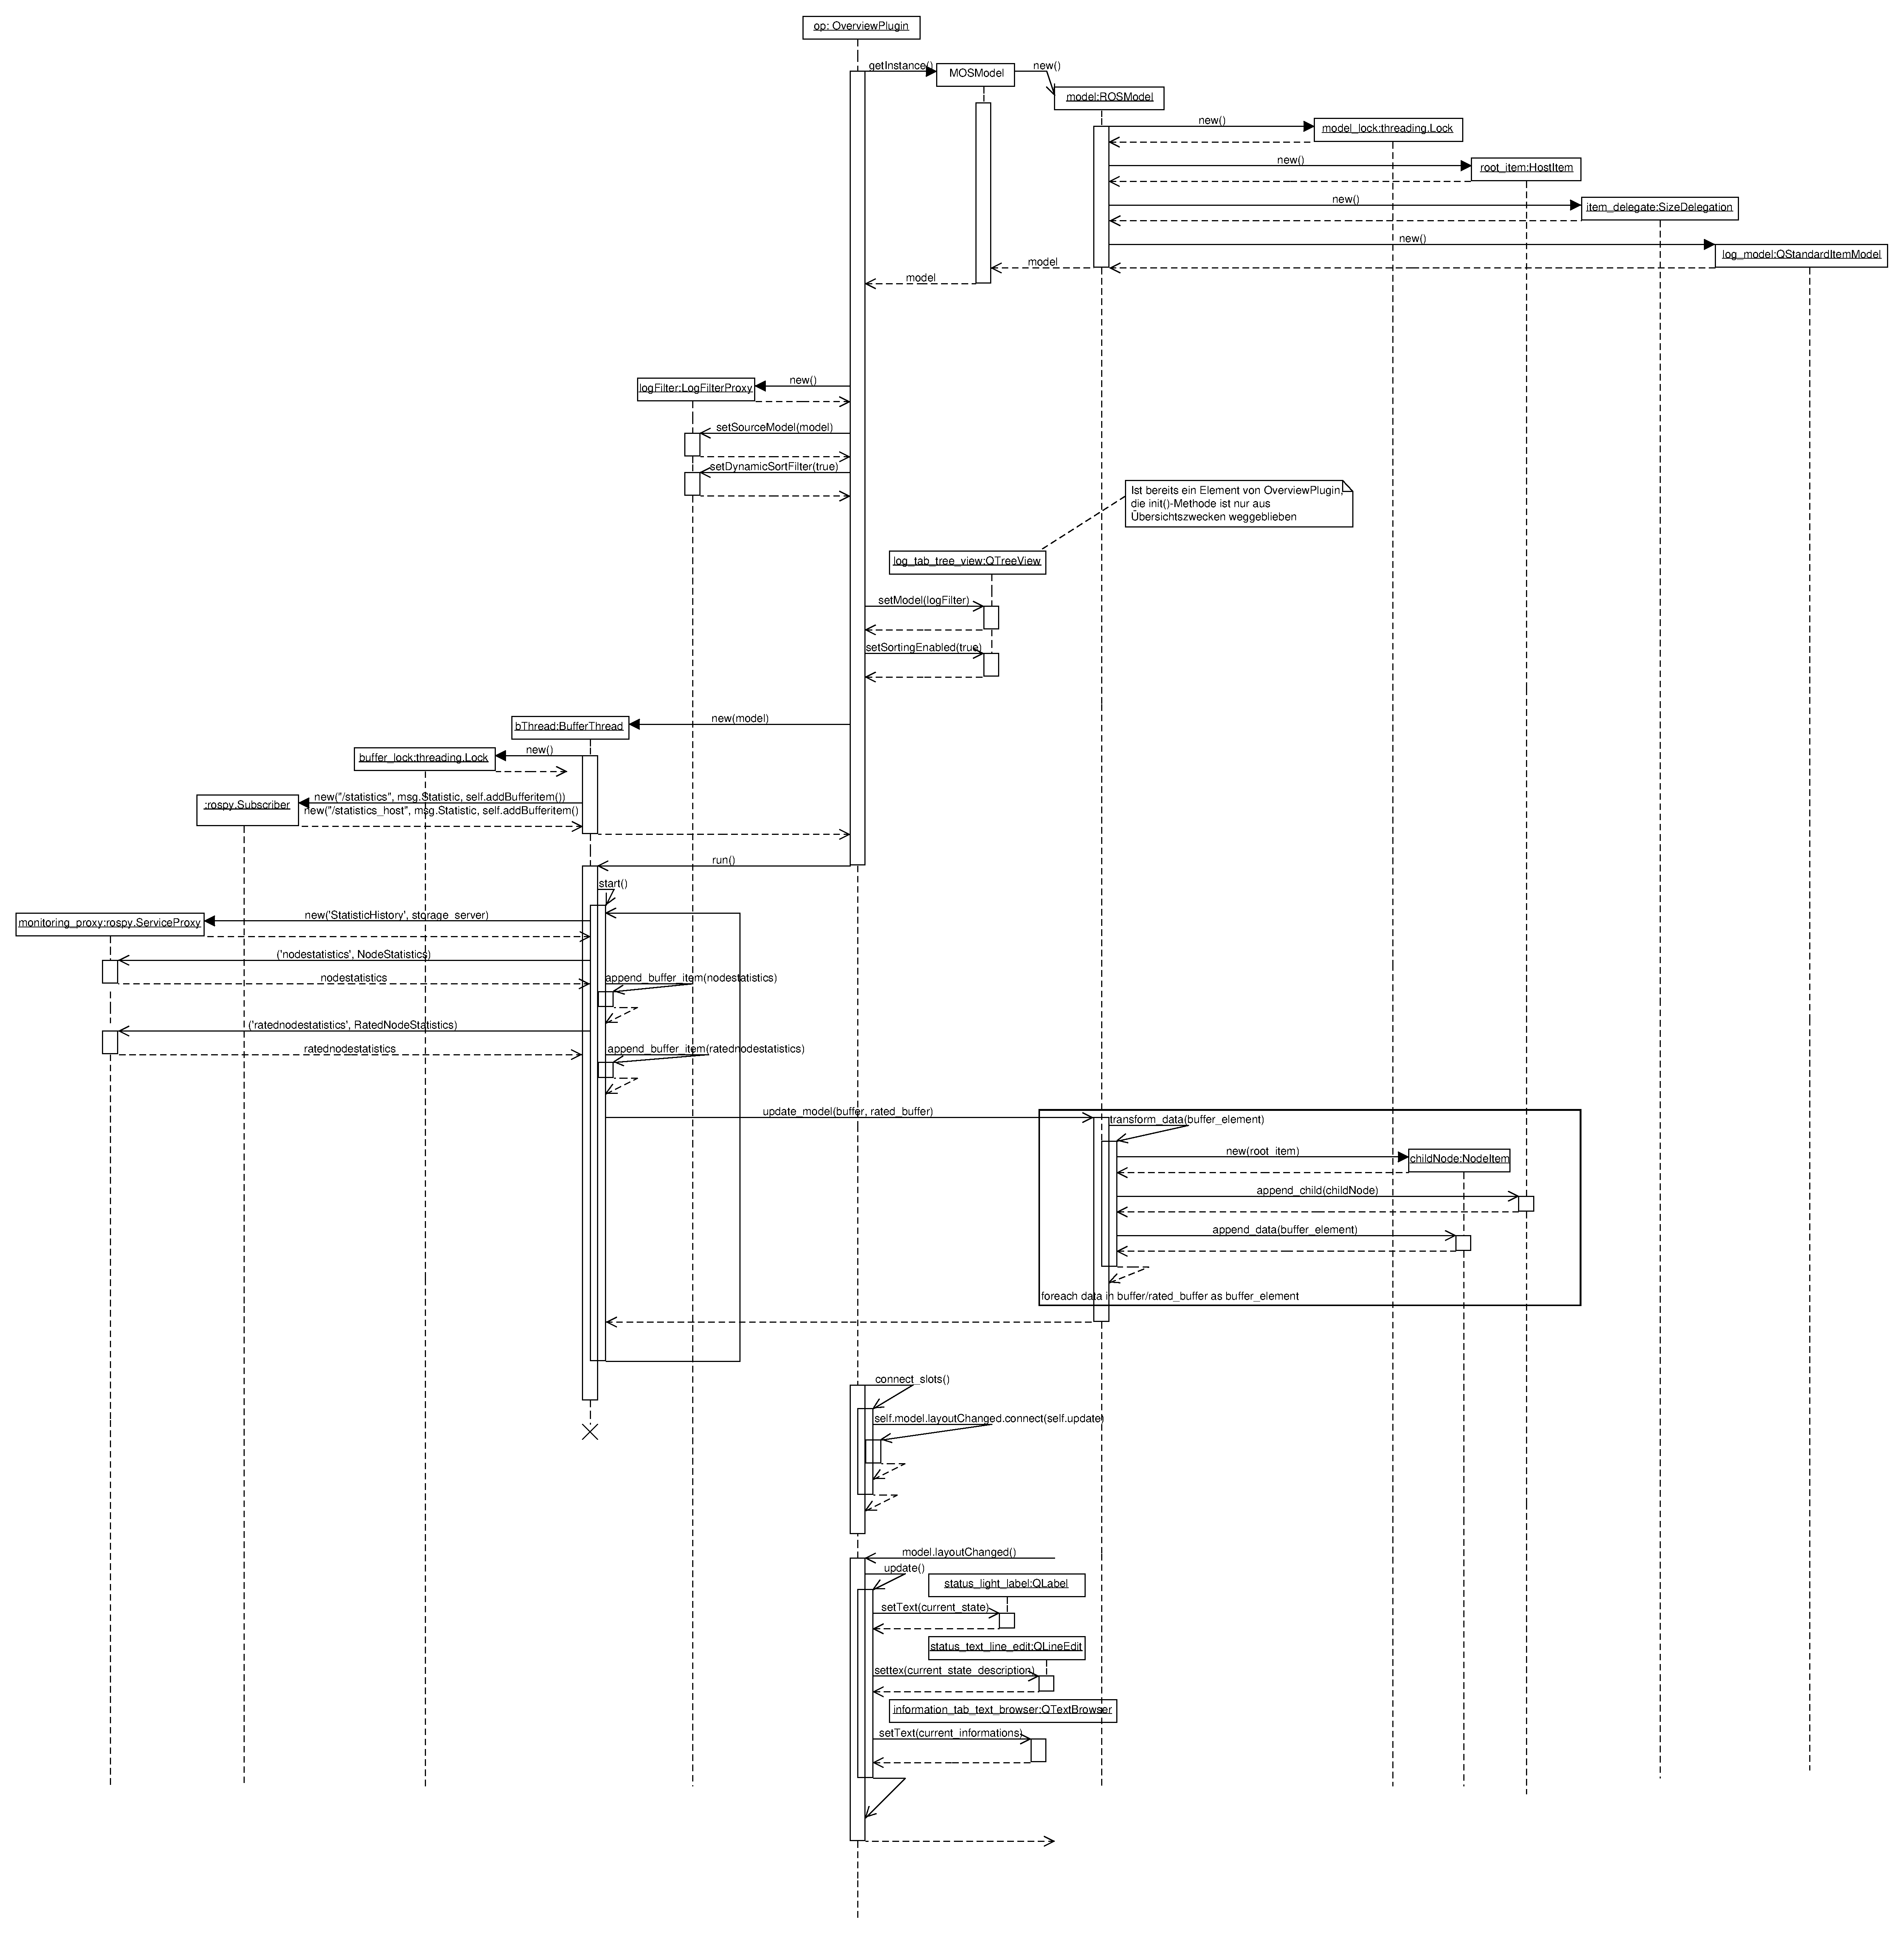
\includegraphics[width=1.0\linewidth]{./diagram_pictures/GUI_seq.pdf}
		\caption{A example GUI sequence.}
	\end{center}
\end{figure}

\subsection*{Setup}
In this sequence diagramm it is exemplary shown how the GUI part of the Software initializes.
All widgets do whenever startet proceed the following steps: Initialize their own data, create or get the model, synchronize with an additional proxy model and then create and start the BufferThread so data is flowing in. The BufferThread then connects via the services to the MonitoringNode and gets a history of the last messages.
Finally the widgets connect their slots so that e.g. the view gets updated when the model changes.

\subsection*{Running}
When the GUI is running everything is getting updated with Qt's signal and slot mechanism. The BufferThread gets all actual data as a Subscriber of all topics and then regularily redirects this data by updating the model. The changes are then transmitted to the view aka the widgets which then show this incoming data.
\\
\\Any other information on how the classes work and interact can often be discovered by looking at the class diagram.